\section*{WU4}
\begin{figure}[here]
	\center
	\caption{wu4: Plot of circular data that are generated with shared center.}
	\label{fig:wu4}
	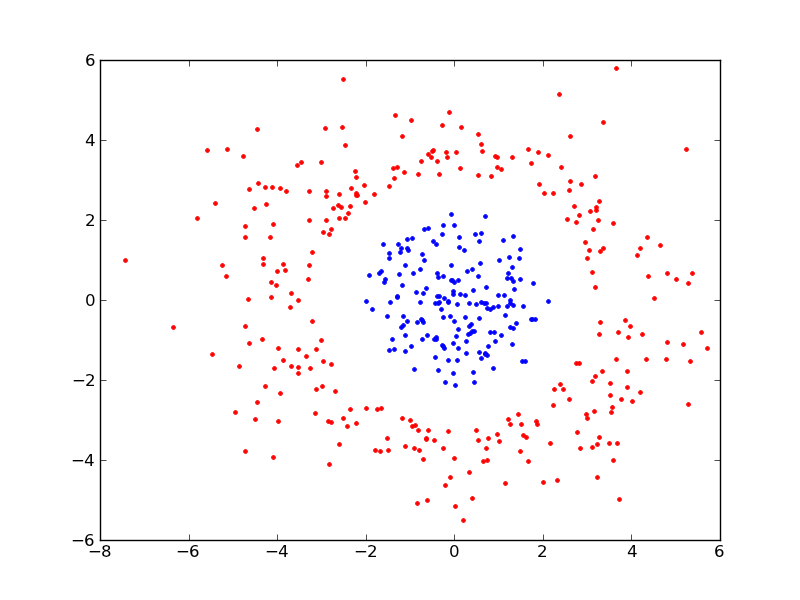
\includegraphics[width=4.0in]{img/wu4.png}
\end{figure}
Figure \ref{fig:wu4} shows the plot of the data. 
Vanilla PCA will find this data difficult because the variance in all directions is similar. This means that eigenvectors can point in any direction.

The large eigenvalues have no significance. For example, with a poly3 kernel, the eigenvalues are ridiculously 
large due to cubing the dot product. What does hold significance, however, is the normalized eigenvalues. 

\section*{WU5}
\begin{figure}[here]
	\center
	\caption{wu5: Plot of data points transformed by vanilla PCA}
	\label{fig:wu5}
	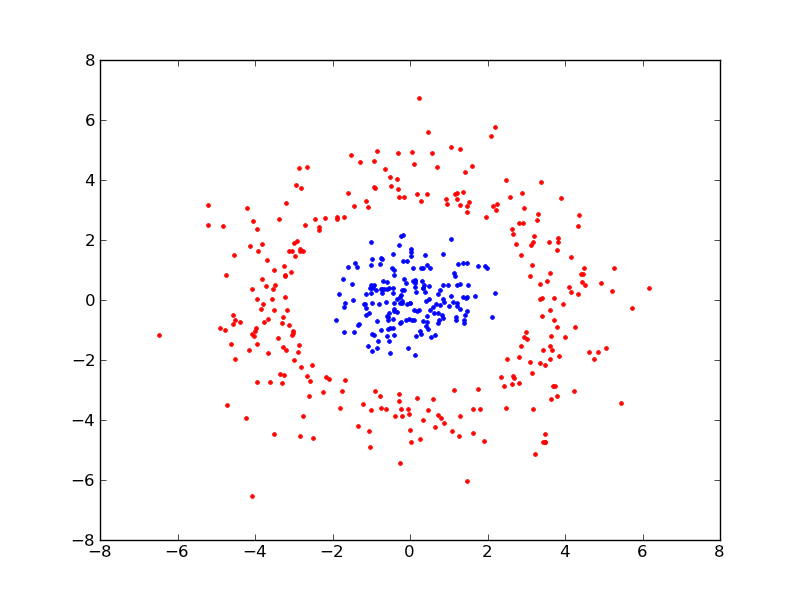
\includegraphics[width=4.0in]{img/wu5.png}
\end{figure}

Figure \ref{fig:wu5} shows the result of PCA. 
PCA did not do what we want it to do :'(
In addition to the reasons listed in WU4, vanilla PCA 
did not do what we wanted to do because the data 
is not linearly separable.

\section*{WU6}
\begin{figure}[here]
	\center
	\caption{wu6: Plot of data points transformed by a rbf1 kernel}
	\label{fig:wu6}
	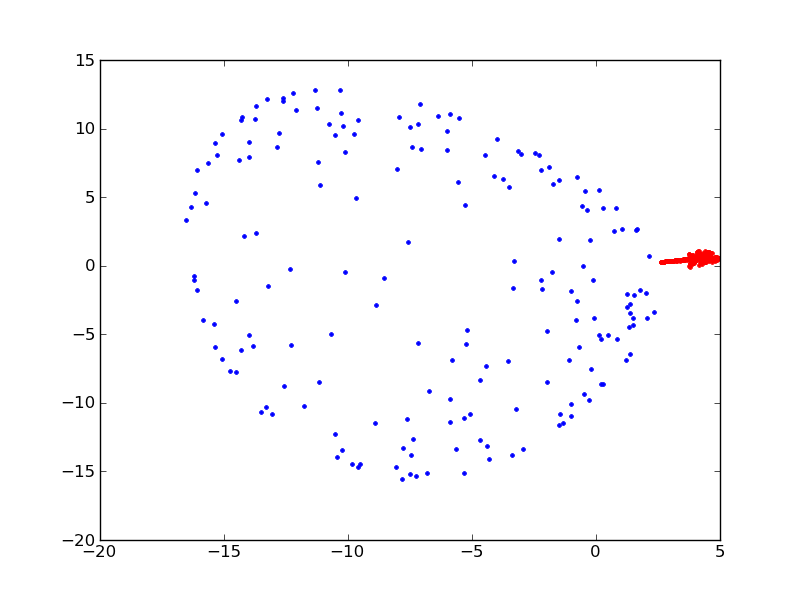
\includegraphics[width=4.0in]{img/wu7_rbf1.png}
\end{figure}

The eigenvalues for KPCA with rbf1 kernel is [ 0.08270371  0.07927822], which is significantly smaller than
the eigenvalues for KPCA with linear kernel: [ 5.68035099  1.51738947]. This means that the rbf1 kernel does a much 
better job at making the data linearly separable than the linear kernel. See the Figure \ref{fig:wu7_rbf1} for a plot of the rbf1 kernel and Figure \ref{fig:wu7_linear} for the plot of the linear kernel for a visual comparison.

\section*{WU7}
\begin{table}[here]
	\centering % used for centering table
	\begin{tabular}{l l l l l} % centered columns (2 columns)
		\hline\hline %inserts double horizontal lines
		Kernel & Top eigen values & Variance & $\lambda_0$ & $\lambda_0 + \lambda_1$  \\ [0.5ex] % inserts table
		%heading
		\hline % inserts single horizontal line
		Linear & (6.163,   5.757) & (3.032E+03,  2.833E+03) & 0.517 & 1. \\ % inserting body of the table
		Poly2 & (6.410E+01,  6.277E+01) & (3.154E+04,  3.088E+04) & 0.312 & 0.618 \\
		Poly3 & (2.906E+03,  2.477E+03) & (1.429E+06,  1.219E+06) & 0.379 & 0.701 \\
		RBF 0.2 & (1.454E-01,  1.008E-01) & (7.153.E+01,   4.959E+01) & 0.176 & 0.297 \\
		RBF 0.5 & (1.122E-01,  6.507E-02) & (5.522E+01,  3.201E+01) & 0.123 & 0.194 \\
		RBF 1 & (7.797E-02,  5.560E-02) & (3.836E+01,  2.735E+01) & 0.082 & 0.140 \\
		RBF 2 & (5.140E-02,  4.200E-02) & (2.529E+01,  2.067E+01) & 0.053 & 0.096 \\
		RBF 5 & (2.830E-02,  2.551E-02) & (1.392E+01  1.255E+01) & 0.029 & 0.055 \\ [1ex] % [1ex] adds vertical space
		\hline %inserts single line
	\end{tabular}
	\label{table:wu7} % is used to refer this table in the text
	\caption{Examples of convergence} % title of Table
\end{table}

Table 1 shows that the linear kernel does the best job in terms of 
getting most variance in the first two principle component. The poly2 kernel and
the poly3 kernel also do good job in getting much of variance with the first two 
principle component.
However, if you look at plotted data points, none of three kernels make
data linearly separable.

On the other hand, RBF kernels make the data linearly separable. Among all RBF kernels, 
RBF 0.2 does the best job in getting as much of the variance on the first two principle 
component.

Plots for the various kernels:
\begin{itemize}
	\item linear: Figure \ref{fig:wu7_linear}
	\item poly2: Figure \ref{fig:wu7_poly2}
	\item poly3: Figure \ref{fig:wu7_poly3}
	\item rbf0.2: Figure \ref{fig:wu7_rbf0_2}
	\item rbf0.5: Figure \ref{fig:wu7_rbf0_5}
	\item rbf2: Figure \ref{fig:wu7_rbf2}
	\item rbf5: Figure \ref{fig:wu7_rbf5}
\end{itemize}


\begin{figure}[here]
	\center
	\caption{wu7: KPCA with a linear kernel}
	\label{fig:wu7_linear}
	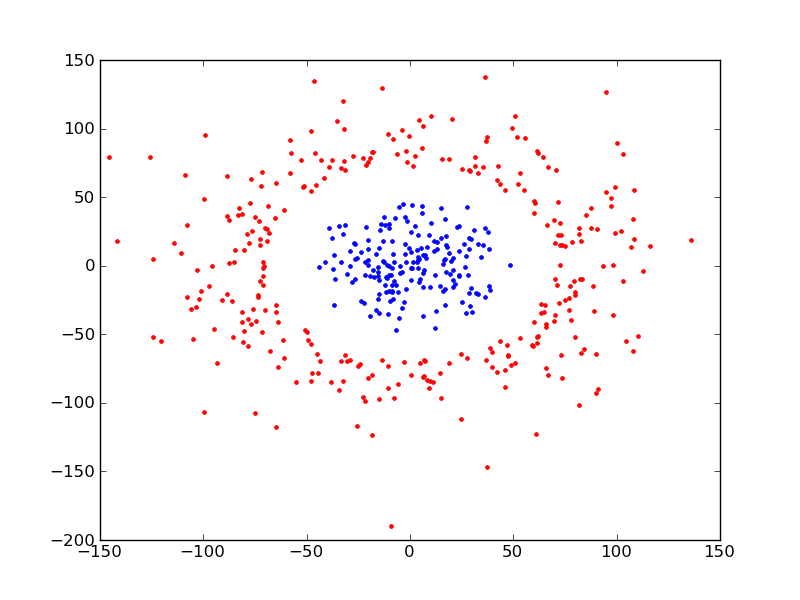
\includegraphics[width=4.0in]{img/wu7_linear.png}
\end{figure}

\begin{figure}[here]
	\center
	\caption{wu7: KPCA with a poly2 kernel}
	\label{fig:wu7_poly2}
	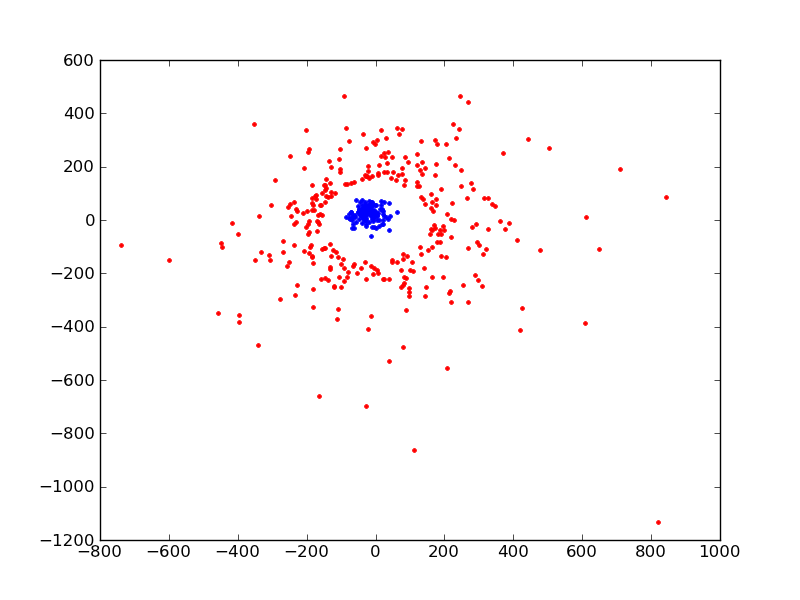
\includegraphics[width=4.0in]{img/wu7_poly2.png}
\end{figure}

\begin{figure}[here]
	\center
	\caption{wu7: KPCA with a poly3 kernel}
	\label{fig:wu7_poly3}
	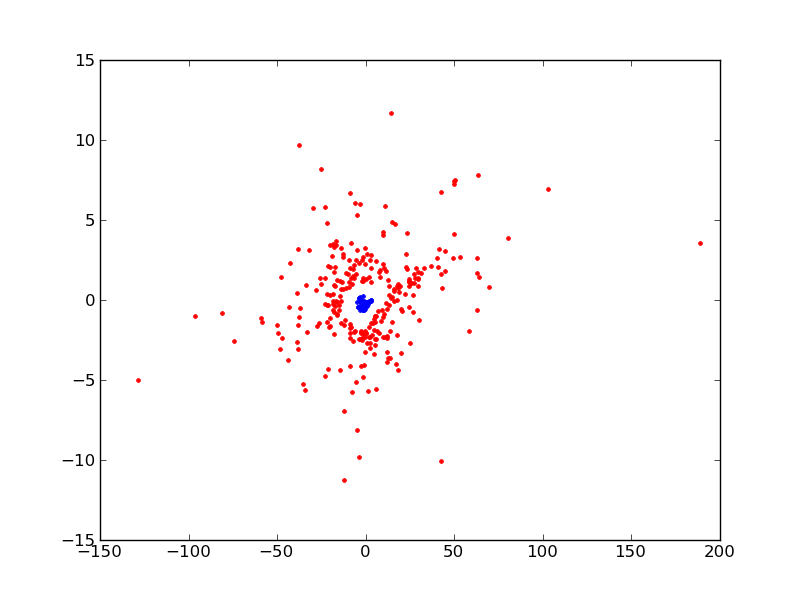
\includegraphics[width=4.0in]{img/wu7_poly3.png}
\end{figure}

\begin{figure}[here]
	\center
	\caption{wu7: KPCA with a rbf0.2 kernel}
	\label{fig:wu7_rbf0_2}
	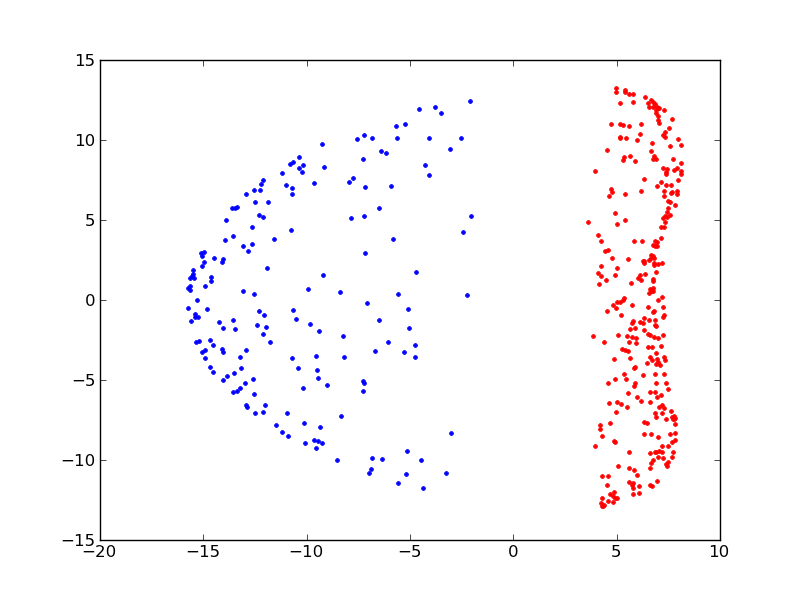
\includegraphics[width=4.0in]{img/wu7_rbf0_2.png}
\end{figure}

\begin{figure}[here]
	\center
	\caption{wu7: KPCA with a rbf0.5 kernel}
	\label{fig:wu7_rbf0_5}
	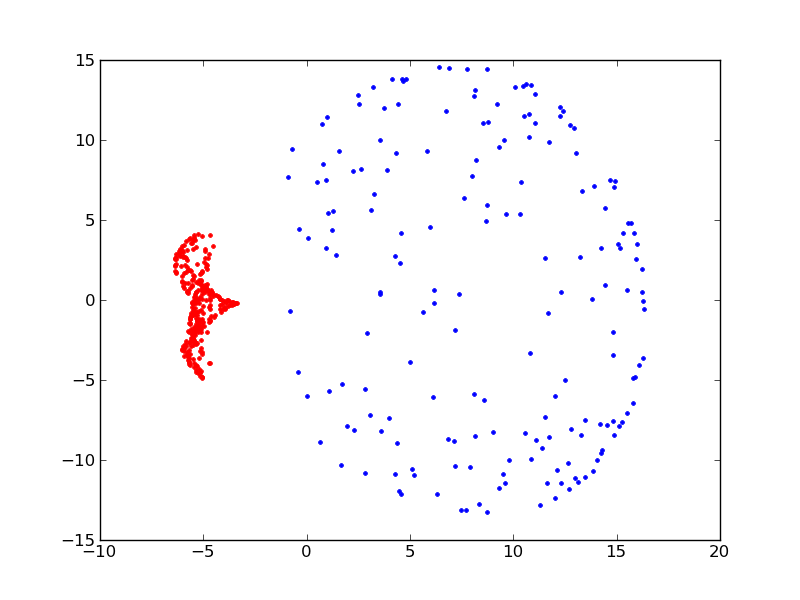
\includegraphics[width=4.0in]{img/wu7_rbf0_5.png}
\end{figure}

\begin{figure}[here]
	\center
	\caption{wu7: KPCA with a rbf1 kernel}
	\label{fig:wu7_rbf1}
	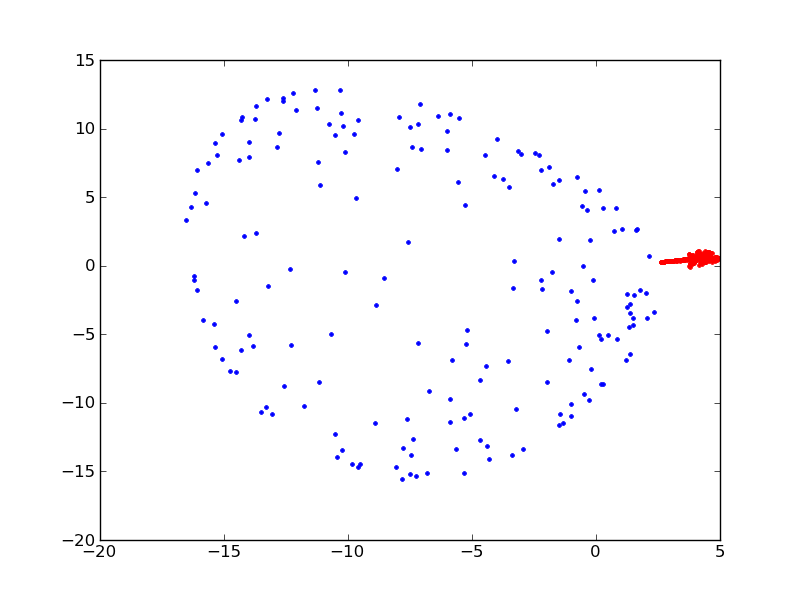
\includegraphics[width=4.0in]{img/wu7_rbf1.png}
\end{figure}

\begin{figure}[here]
	\center
	\caption{wu7: KPCA with a rbf2 kernel}
	\label{fig:wu7_rbf2}
	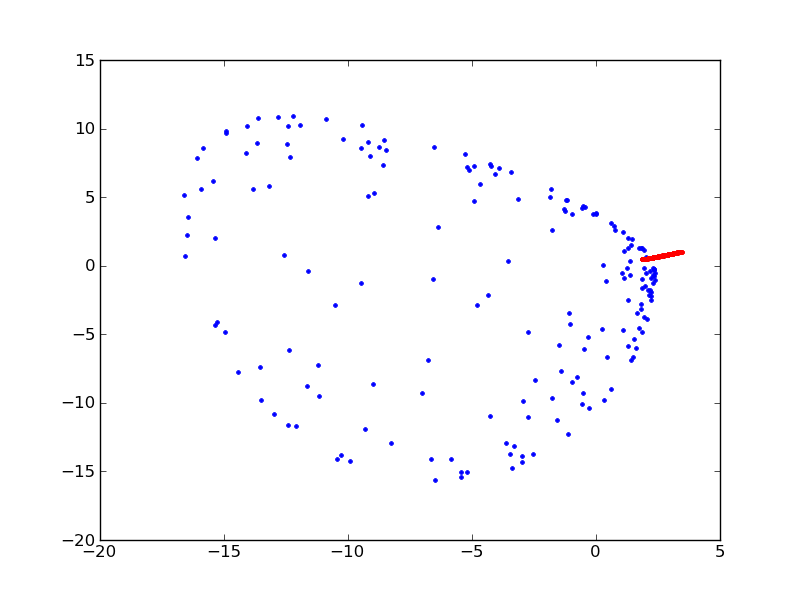
\includegraphics[width=4.0in]{img/wu7_rbf2.png}
\end{figure}

\begin{figure}[here]
	\center
	\caption{wu7: KPCA with a rbf5 kernel}
	\label{fig:wu7_rbf5}
	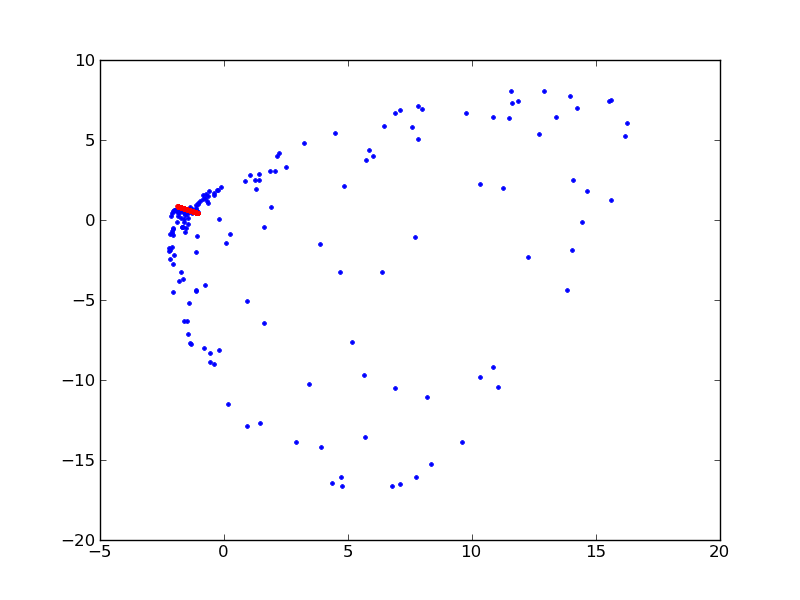
\includegraphics[width=4.0in]{img/wu7_rbf5.png}
\end{figure}